\documentclass{../praktikum-ppt}
\usepackage{tikz-3dplot}

\author[Tew \& Haf]{Teosofi Hidayah Agung \\ Hafidz Mulia}
\date{19 Mei 2025}
\title[Alpro 2 - Week 8]{\textit{Inheritance} \& \textit{Polymorphism}}
\institute[Matematika ITS]{Departemen Matematika\\ Institut Teknologi Sepuluh Nopember}

\begin{document}

{\usebackgroundtemplate{
  \tikz[overlay,remember picture] \node[opacity=0.2, at=(current page.center)]{\includegraphics[width=\paperwidth]{bg_22}};}
\begin{frame}
  \titlepage
\end{frame}
}

\AtBeginSection{
    {\usebackgroundtemplate{
     \tikz[overlay,remember picture] \node[opacity=0.1, at=(current page.center)]{\includegraphics[width=\paperwidth]{code_bg}};}
    \begin{frame}{Daftar isi}
        \tableofcontents[currentsection]
        % \begin{tikzpicture}[overlay, remember picture] 
        %     \node at ([yshift=.5cm]current page.south east) [
        %         anchor = south east, 
        %         ] {
        %     \animategraphics[autoplay,loop,width=0.2\textwidth]{30}{Arisu Dance/Arisu Dance-}{0}{186}
        %     };
        % \end{tikzpicture}
    \end{frame}}
    }

    \begin{frame}
      \centering
      \begin{tikzpicture}[every node/.style={scale=0.7}]
  % Zombie class
  \umlclass[x=-3,y=0]{Zombie}{
    - HP : int
  }{
    \# Zombie()\\
    \# Zombie(int hp)\\
    $\sim$ setHP(int hp)\\
    $\sim$ getHP() : int\\
    + walk() : void\\
    + attack() : void\\
    + voice() : void
  }

  % Villager class
  \umlclass[x=3.5,y=0]{Villager}{
    - profession : String\\
    - HP : int
  }{
    \# Villager()\\
    \# Villager(String job, int hp)\\
    + walk() : void\\
    + trade() : void\\
    + voice() : void
  }

  % Creeper class
  \umlclass[x=0,y=0]{Creeper}{
    - HP : int
  }{
    \# Creeper()\\
    \# Creeper(int hp)\\
    $\sim$ setHP(int hp)\\
    $\sim$ getHP() : int\\
    + walk() : void\\
    + explode() : void\\
    + voice() : void\\
  }
  \end{tikzpicture}

        \begin{masalah}
          Menurut kalian struktur class seperti diatas apakah sudah efisien/sederhana? Jika masih belum, bagaimana cara agar pembuatan class diatas lebih efisien?
        \end{masalah}
    \end{frame}

    \section{Inheritance}
    \begin{frame}{\insertsection}
        \begin{definisi}
            \textbf{Inheritance} adalah sebuah konsep dalam pemrograman berorientasi objek yang memungkinkan sebuah kelas untuk mewarisi atribut dan metode dari kelas lain. Kelas yang mewarisi disebut sebagai \textit{subclass} atau \textit{child class}, sedangkan kelas yang diwarisi disebut sebagai \textit{superclass} atau \textit{parent class}. 
        \end{definisi}
        \begin{figure}[h!]
          \centering
          \begin{tikzpicture}[every node/.style={scale=0.8}]
  % Parent class
  \umlclass[x=0, y=0]{Parent}{}{}

  % Child classes
  \umlclass[x=-2, y=-2]{ChildA}{}{}
  \umlclass[x=0, y=-2]{ChildB}{}{}
  \umlclass[x=2, y=-2]{ChildC}{}{}

  % Inheritance arrows
  \umlinherit[geometry=|-|]{ChildA}{Parent}
  \umlinherit[]{ChildB}{Parent}
  \umlinherit[geometry=|-|]{ChildC}{Parent}
\end{tikzpicture}
          \caption{Struktur inheritance}       
        \end{figure}
    \end{frame}

    \begin{frame}{\insertsection}
        \begin{block}{Manfaat}
            \begin{itemize}
                \item Mengurangi duplikasi kode
                \item Memudahkan pemeliharaan kode
                \item Memungkinkan penggunaan polymorphism
            \end{itemize}
        \end{block}
        \begin{alertblock}{Catatan}
          Sama seperti anak yang hanya memiliki satu ibu kandung, subclass hanya dapat mewarisi dari satu superclass. Disisi lain superclass dapat memiliki banyak subclass.
        \end{alertblock}
    \end{frame}

    \begin{frame}[fragile]{\insertsection}
        \begin{lstlisting}[caption={Struktur syntax inheritance}]
  class Parent {
      void display() {
          System.out.println("This is the Parent class");
      }
  }

  class Child extends Parent {
      void display() {
          System.out.println("This is the Child class");
      }
  }
        \end{lstlisting}
    \end{frame}

    \begin{frame}{\insertsection}
        \begin{figure}[h!]
          \centering
          \caption{Efesiensi struktur class}
          \begin{tikzpicture}[every node/.style={scale=0.7}]
  % Mob class
  \umlclass[x=0,y=0]{Mob}{
    - HP : int
  }{
    \# Mob()\\
    \# Mob(int hp)\\
    $\sim$ setHP(int hp)\\
    $\sim$ getHP() : int\\
    + walk() : void\\
    + voice() : void
  }
  % Zombie class
  \umlclass[x=4,y=-2]{Zombie}{}{
    + attack() : void
  }

  % Villager class
  \umlclass[x=4,y=0]{Villager}{
    - profession : String
  }{
    + trade() : void
  }

  % Creeper class
  \umlclass[x=4,y=2]{Creeper}{}{
    + explode() : void
  }

  % Inheritance arrows
  \umlinherit[geometry=-|-]{Zombie}{Mob}
  \umlinherit[]{Villager}{Mob}
  \umlinherit[geometry=-|-]{Creeper}{Mob}
  \end{tikzpicture}
        \end{figure}
    \end{frame}

    \subsection{Constructor Child Class}
    \begin{frame}{\insertsection}
      \framesubtitle{\insertsubsection}
        \begin{block}{Constructor Child Class}
            \begin{itemize}
                \item Constructor child class akan memanggil constructor parent class
                \item Jika constructor parent class tidak ada, maka constructor child class tidak dapat diakses
            \end{itemize}
        \end{block}
        Biasanya constructor parent class dipanggil dengan menggunakan keyword \texttt{super()}. Method ini harus dipanggil ketika parent class punya konstruktor dengan parameter atau ketika mau memanggil method atau atribut dari parent class yang di-override di child class.
  \end{frame}
    \begin{frame}[fragile]{\insertsection}
      \framesubtitle{\insertsubsection}
        \begin{lstlisting}[caption={Contoh constructor child class}]
  class Parent {
      int x;
      Parent(int x) {
          this.x = x;
      }
  }
  class Child extends Parent {
      int y;
      Child(int x, int y) {
          super(x); // Memanggil constructor Parent
          this.y = y;
      }
  }
        \end{lstlisting}
    \end{frame}

    \section{Polymorphism}
    \begin{frame}{\insertsection}
        \begin{definisi}
            \textbf{Polymorphism} adalah kemampuan suatu objek untuk memiliki banyak bentuk. Dalam konteks pemrograman berorientasi objek, polymorphism memungkinkan kita untuk menggunakan metode yang sama pada objek yang berbeda, meskipun implementasinya berbeda.
        \end{definisi}
        Intinya sebuah objek induk bisa memanggil method yang ada pada kelas anaknya. Misalkan kita punya class induk \texttt{Hewan} dan class anak \texttt{Sapi}. Kita bisa memanggil method yang ada di class \texttt{Sapi} dengan menggunakan objek dari class \texttt{Hewan}. Contohnya seperti berikut:
    \end{frame}

    \begin{frame}[fragile]{\insertsection}
        \begin{lstlisting}[caption={Contoh polymorphism}]
  class Parent {
      void method1() {
          System.out.println("Parent method");
      }
  }
  class Child extends Parent {
      void method1() {
          System.out.println("Child method");
    }
  }
  class Main {
    public static void main(String[] args) {
        Parent obj = new Child(); // Polymorphism
        obj.method1(); // Error: methodChild() not found
    }
  }
        \end{lstlisting}
      
    \end{frame}


    \begin{frame}{\insertsection}
      Sekarang coba ingat kembali tentang materi Logika Matematika. Misalkan aku mempunyai kalimat kebenaran:
      \begin{quote}
        \centering\color{red}
        ``Semua sapi adalah Hewan''
        \[\forall x (S(x) \implies H(x))\]
      \end{quote}
      Sekarang ketika aku bilang "Semua sapi itu pasti hewan", apakah itu benar? \onslide<2->{\textbf{Ya, jelas benar}. Sekarang coba kita ubah kalimatnya menjadi "Semua hewan adalah sapi". Apakah itu benar? \onslide<3->{\textbf{Tidak, jelas itu kurang tepat}.}}
    \end{frame}

    \begin{frame}[fragile]{\insertsection}
      \begin{contoh}
        Misal kita punya class \texttt{Hewan} dan class anaknya adalah \texttt{Sapi}, \texttt{Kucing}, dan \texttt{Ayam}. 
      \end{contoh}
      \begin{lstlisting}[caption={Aplikasi polymorphism}]
    Hewan[] hewan2 = { new Sapi(), new Kucing(), new Ayam() };
        
    for (Hewan h : hewan2) {
      h.bersuara();
    }
        \end{lstlisting}
    \end{frame}

    \begin{frame}[fragile]{\insertsection}
      \begin{contoh}
        Atau misal dalam \textit{minecraft} dimana kita dapat mengatur difficulty dari game tersebut.
      \end{contoh}
      \begin{lstlisting}[caption={Aplikasi dalam game}]
    Mob[] mobs = {new Villager(),new Zombie(),new Creeper()};
    
    for (Mob m : mobs) {
      if (difficulty.equals("peaceful") && (m instanceof Zombie || m instanceof Creeper)) {
          continue;
      } else {
          m.spawn();  
      }
    }
      \end{lstlisting}
    \end{frame}
    
    \section{Diagram Kelas}
    \subsection{Hubungan/Relasi}
    \begin{frame}{\insertsection}
      \framesubtitle{\insertsubsection}
      \begin{block}{Hubungan/Relasi}
        \begin{itemize}
          \item Pewarisan : hubungan antara dua class di mana satu class mewarisi atribut dan metode dari class lain.
          \item Implementasi : hubungan antara class dan interface di mana class mengimplementasikan method yang didefinisikan dalam interface.
        \end{itemize}
        \begin{alertblock}{Catatan}
          Sebenarnya cukup banyak relasi yang ada dalam diagram kelas, tetapi kita hanya akan membahas dua relasi ini saja.
        \end{alertblock}
      \end{block}
    \end{frame}

    \begin{frame}{\insertsection}
      \framesubtitle{\insertsubsection}
      \begin{figure}[h!]
        \centering
        \begin{tikzpicture}[every node/.style={scale=0.7}]
  % Parent class
  \umlclass[x=2, y=0]{Parent1}{}{}
  \umlclass[x=-2, y=0]{Parent2}{}{}
  % Child class
  \umlclass[x=4, y=0]{Child1}{}{}
  \umlclass[x=-4, y=0]{Child2}{}{}
  % Interface
  \umlinterface[x=0, y=2]{Interface}{}{}
  % Inheritance arrows
  \umlinherit[]{Child1}{Parent1}
  \umlinherit[]{Child2}{Parent2}
  % Implementation arrows
  \umlreal[geometry=|-]{Parent1}{Interface}
  \umlreal[geometry=|-]{Parent2}{Interface}
  \end{tikzpicture}
        \caption{Hubungan/Relasi}
      \end{figure}
      \begin{contoh}
        \begin{itemize}
          \item Pewarisan : class \texttt{Child} mewarisi atribut dan metode dari class \texttt{Parent}.
          \item Implementasi : class \texttt{Child} mengimplementasikan metode yang didefinisikan dalam interface \texttt{Interface}.
        \end{itemize}
      \end{contoh}
    \end{frame}

    \section{Latihan}
    \begin{frame}
      \begin{latihan}
        Buatlah class dalam \textit{Java} yang merepresentasikan diagram kelas berikut:
      \end{latihan}
      \begin{figure}[h!]
        \centering
        \begin{tikzpicture}[every node/.style={scale=0.7}]
  % Parent class
  \umlclass[x=0, y=0]{Node}{
    - data : int
  }{
    + Node(int data)\\
    + getData() : int\\
    + setData(int data) : void
  }
  % Child classes
  \umlclass[x=6, y=0]{BinaryNode}{
    - left : Node\\
    - right : Node
  }{
    + BinaryNode(int data, Node left, Node right)\\
    + getLeft() : Node\\
    + getRight() : Node
  }
  \umlinherit[]{BinaryNode}{Node}
        \end{tikzpicture}
      \end{figure}
      
    \end{frame}
\end{document}